\section{Wstęp}

Celem projektu było stworzenie aplikacji serwerowej dla obiektu Internetu Rzeczy działającej w~oparciu o~autorską lub dostępną publicznie implementację protokołu CoAP (ang. \textit{Constrained Application Protocol}). Platformą docelową został moduł \mbox{\textbf{NodeMCU}} w~wersji trzeciej wyposarzony w~układ SoC ESP8266 oraz 4MiB pamięci Flash dołączonej za pośrednictwem interfejsu Quad SPI. Niewątpliwą zaletą urządzenia jest zintegrowany moduł WiFi w~standardzie 802.11b/g/n. Na płytce umieszczony został układ CH340 umożliwiający komunikację z~wykorzystaniem protokołu USB $\leftrightarrow$ UART.

\begin{figure}[h]
    \centering
    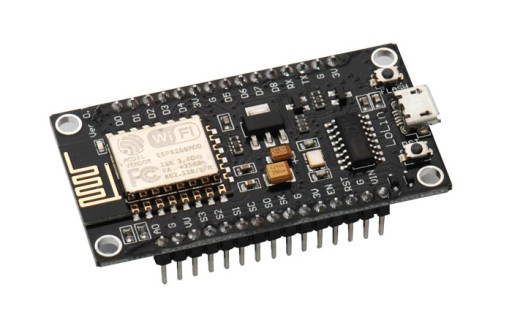
\includegraphics[scale=0.6]{img/esp8266.jpg}
    \label{esp8266}
    \caption{Płytka rozwojowa NodeMCU w~wersjii trzeciej}
\end{figure}
\vspace{0.5cm}

Istnieją dwie zasadnicze możliwości programowania układów z~rodziny ESP. Pierwsza z~nich to dostosowany do możliwości platformy interfejs Arduino. Dostępny jest on do pobrania z~poziomu Arduino IDE i~umożliwia wykorzystanie bogatego zbioru bibliotek tworzonego przez społeczność zgromadzoną wokół platformy. Drugą z~opcji jest posłużenie się dostarczanym przez producenta układu ESP8266 - firmę Espressif - zbiorem narzędzi dystrybuowanym pod nazwą ESP8266-RTOS-SDK \cite{sdk}. Poza kompilatorem, skryptami linkera oraz implementacją biblioteki standardowej C~SDK dostarcza także całą gamę sterowników, implementacji popularnych protokołów komunikacyjnych i~szyfrujących a~także narzędzia umożliwiające sprawne zarządzanie projektem oraz debugowanie. Ze względu na osobiste preferencje autorów w~projekcie zdecydowano się wykorzystać platformę SDK. Prace na projektem podzielono na cztery etapy:

\begin{enumerate}
    \item implementacja protokołu
    \item stworzenie aplikacji serwerowej
    \item opracowanie i~przeprowadzenie testów
    \item stworzenie dokumentacji
\end{enumerate}

Ostatecznym efektem projektu jest oprogramowanie spełniające wszystkie postawione przed nim wymagania funkcjonalne. 